\section{Experiments}\label{sec:experiments}
In this work, we take four applications including matrix multiplication (MM), FIR filter, Kmean and Sobel edge detector as our benchmark. In order to be more representative, each application is further provided with three different data sets ranging from small, medium to large ones. The basic parameters and configurations of the benchmark is explained in the \tabref{tab:benchmark-config}.

\begin{table*}[t]
  \caption{Detailed Configurations of the Benchmark}
  \label{tab:benchmark-config}
  \centering
  \begin{tabular}{c|c|c|c|c}
  \hline
  Benchmark & MM & FIR & Sobel & Kmean \\ \hline
  Parameters & Matrix Size & \tabincell{c}{\# of Input \\ \# of Taps+1} & \tabincell{c}{ \# of Vertical Pixels \\ \# of Horizontal Pixels} & \tabincell{c}{\# of Nodes \\ \# of Centroids \\ Dimension Size} \\ \hline
  Small & 10 & 40/50 & 8/8 & 20/4/2 \\ \hline
  Medium & 100 & 10000/50 & 128/128 & 5000/4/2  \\ \hline
  Large & 1000 & 100000/50 & 1024/1024 & 50000/4/2 \\ \hline
  \end{tabular}
\end{table*}


The benchmark is implemented on Zedboard using both Vivado HLS and QuickDough to build the FPGA acceleration system. Then design productivity, implementation efficiency and performance of the two design methods are compared respectively.

\subsection{Experiment Setup}
All the runtimes were obtained from a computer with Intel(R) Core(TM) i5-3230M CPU and 8GB RAM. Vivado HLS 2013.3 is used to transform the compute kernel to hardware IP Catalog. Vivado 2013.3 is then used to integrate the IP core and build the FPGA accelertor on Zedboard. The SCGRA is initially built using ISE 14.7 and then exported as an IP core. Afterwards, it is integrated into the SCGRA based FPGA accelerator using PlanAhead 14.7. Finally, the accelerators are implemented on Zedboard to run the benchmark on bare-metal system mode.

Vivado HLS typically achieves the trade-off between hardware overhead and performance through altering the loop unrolling factor and loop blocking size. Larger block size is beneficial to data reuse and amortizing the communication cost, but it is usually constrained by the size of on-chip buffer. Similarly, larger loop unrolling factor typically promises better performance, however, hardware resources like DSP blocks will soon be used up and implementation frequency will degrade as well. In this work, two different sets of input/output buffer configurations are applied for the Vivado HLS based acceleration design. One set has fixed 2k-word buffer for both input and output, and the other set has maximum available buffer size and it could use as much as 64k-word for both input and output. \tabref{tab:loop-unrolling-setup-vivado} shows the near optimal blocking and loop unrolling setup for the benchmark. 

\begin{table*}[t]
\centering
\caption{Loop Unrolling \& Blocking Setup for Vivado HLS Based Accelerator Design}
\label{tab:loop-unrolling-setup-vivado}
\begin{tabular}{|l|l|l|l|l|l|l|}
\hline
\multicolumn{2}{|l|}{\multirow{2}{*}{Application}} & \multicolumn{2}{l|}{Max-Buffer} & \multicolumn{2}{l|}{2k-Buffer} & \multirow{2}{*}{Complete Loop Structure} \\ \cline{3-6}
\multicolumn{2}{|l|}{} & Unrolling Factor & Block Structure & Unrolling Factor & Block Structure & \\ \hline
\multirow{3}{*}{MM} & Small & $2 \times 10 \times 10$ & $10 \times 10 \times 10$ & $2 \times 10 \times 10$ & $10 \times 10 \times 10$ & $10 \times 10 \times 10$ \\ \cline{2-7} 
                    & Medium & $1 \times 1 \times 100$ & $100 \times 100 \times 100$ & $1 \times 100$ & $10 \times 100$ & $100 \times 100 \times 100$ \\ \cline{2-7} 
                    & Large & $1 \times 500$ & $50 \times 1000$ & 500 & 1000  & $1000 \times 1000 \times 1000$ \\ \hline
\multirow{3}{*}{FIR} & Small & $2 \times 50$ & $40 \times 50$ & $2 \times 50$ & $40 \times 50$ & $40 \times 50$ \\ \cline{2-7} 
                     & Medium & $2 \times 50$ & $10000 \times 50$ & $2 \times 50$ & $1000 \times 50$ & $10000 \times 50$ \\ \cline{2-7} 
                     & Large & $2 \times 50$ & $50000 \times 50$ & $2 \times 50$ & $1000 \times 50$ & $100000 \times 50$ \\ \hline
\multirow{3}{*}{Sobel} & Small & $1 \times 2 \times 3 \times 3$ & $8 \times 8 \times 3 \times 3$ & $1 \times 2 \times 3 \times 3$ & $8 \times 8 \times 3 \times 3$ & $8 \times 8 \times 3 \times 3$ \\ \cline{2-7} 
                       & Medium & $1 \times 1 \times 3 \times 3$ & $128 \times 128 \times 3 \times 3$ & $1 \times 1 \times 3 \times 3$ & $23 \times 128 \times 3 \times 3$ & $128 \times 128 \times 3 \times 3$ \\ \cline{2-7} 
                       & Large & $1 \times 1 \times 3 \times 3$ & $75 \times 1024 \times 3 \times 3$ & $1 \times 1 \times 3 \times 3$ & $4 \times 1024 \times 3 \times 3$ & $1024 \times 1024 \times 3 \times 3$ \\ \hline
\multirow{3}{*}{KMean} & Small & $20 \times 4 \times 2$ & $20 \times 4 \times 2$ & $20 \times 4 \times 2$ & $20 \times 4 \times 2$ & $20 \times 4 \times 2$ \\ \cline{2-7} 
                       & Medium & $5 \times 4 \times 2$ & $5000 \times 4 \times 2$ & $5 \times 4 \times 2$ & $1000 \times 4 \times 2$ & $1000 \times 4 \times 2$ \\ \cline{2-7} 
                       & Large & $5 \times 4 \times 2$ & $25000 \times 4 \times 2$ & $5 \times 4 \times 2$ & $1000 \times 4 \times 2$ & $1000 \times 4 \times 2$ \\ \hline
\end{tabular}
\end{table*}

SCGRA based FPGA accelerator has similar design chocies to that of Vivado HLS in terms of loop unrolling and blocking. The difference is that the unrolled part of the loop is transformed to DFG which is further scheduled to the SCGRA infrastructure, and the loop unrolling factor is limited by the resources of the SCGRA overlay such as SCGRA size, instruction memory size and data memory size. While the block size is contrained by both the size of input/output buffer and the addr buffer. Currently, we set the data buffer to be 2k-word and addr buffer to be 4k-word. However, addr buffer size is the major constrain of the blocking size as useless addresses are also stored. In this work, both a 2x2 SCGRA and 5x5 SCGRA overlay are used for all these benchmark implementation. \tabref{tab:scgra-config} and \tabref{tab:loop-unrolling-setup-scgra} present the detailed SCGRA overlay configuration and loop unrolling as well as blocking of the benchmark respectively.

\begin{table}[h]
\caption{SCGRA Configuration}
\label{tab:scgra-config}
\centering
\begin{tabular}{|l|l|}

\hline
{SCGRA Topology} & {Torus} \\ \hline
{SCGRA Size} & {$2 \times 2$, $5 \times 5$} \\ \hline
{Data Wdith} & {32 bits} \\ \hline
{Instruction Length} & {72 bits} \\ \hline
{Instruction Memory Depth} & {1024} \\ \hline
{Data Memory Depth} & {256} \\ \hline
{Input/Output Buffer Depth} & {2048} \\ \hline
{Addr Buffer Depth} & {4096} \\ \hline

\end{tabular}
\end{table}

\begin{table*}[t]
\centering
\caption{Loop Unrolling and Blocking Setup for SCGRA Based FPGA Accelerator Design}
\label{tab:loop-unrolling-setup-scgra}
\begin{tabular}{|l|l|l|l|l|l|l|l|l|}
\hline
\multicolumn{2}{|l|}{\multirow{2}{*}{Application}} & \multicolumn{3}{l|}{SCGRA 2x2} & \multicolumn{3}{l|}{SCGRA 5x5} & \multirow{2}{*}{Complete Loop Structure} \\ \cline{3-8}
\multicolumn{2}{|l|}{} & Unrolling Factor & DFG(OP/IO) & Block Structure & Unrolling Factor & DFG(OP/IO) & Block Structure & \\ \hline
\multirow{3}{*}{MM} & Small & $10 \times 10 \times 10$ & 1000/301 & $10 \times 10 \times 10$ & $10 \times 10 \times 10$ & 1000/301 & $10 \times 10 \times 10$ & $10 \times 10 \times 10$ \\ \cline{2-9} 
            & Medium & $5 \times 100$ & 750/606 & $10 \times 100$ & $5 \times 100$ & 750/606 & $10 \times 100$ & $100 \times 100 \times 100$ \\ \cline{2-9} 
            & Large & 200 & 301/402 & 1000 & 200 & 301/402 & $10 \times 100$ & $1000 \times 1000 \times 1000$ \\ \hline
\multirow{3}{*}{FIR} & Small & $40 \times 50$ & 860/131 & $40 \times 50$ & $40 \times 50$ & 860/131 & $40 \times 50$ & $40 \times 50$ \\ \cline{2-9} 
                  & Medium & $20 \times 50$ & 1000/141 & $100 \times 50$ & $50 \times 50$ & 2500/201 & $250 \times 50$ & $10^4 \times 50$ \\ \cline{2-9} 
                  & Large & $20 \times 50$ & 1000/141 & $100 \times 50$ & $50 \times 50$ & 2500/201 & $250 \times 50$ & $10^5 \times 50$ \\ \hline
\multirow{3}{*}{Sobel} & Small & $4 \times 8 \times 3 \times 3$ & 1080/39 & $8 \times 8 \times 3 \times 3$ & $8 \times 8 \times 3 \times 3$ & 2160/55 & $8 \times 8 \times 3 \times 3$ & $8 \times 8 \times 3 \times 3$  \\ \cline{2-9} 
                  & Medium & $4 \times 8 \times 3 \times 3$ & 1080/39 & $8 \times 8 \times 3 \times 3$ & $23 \times 8 \times 3 \times 3$ & 6210/115 & $65 \times 8 \times 3 \times 3$ & $128 \times 128 \times 3 \times 3$ \\ \cline{2-9} 
                  & Large & $4 \times 4 \times 3 \times 3$ & 540/31 & $16 \times 4 \times 3 \times 3$ & $16 \times 4 \times 3 \times 3$ & 2160/55 & $16 \times 4 \times 3 \times 3$ & $1024 \times 1024 \times 3 \times 3$  \\ \hline
\multirow{3}{*}{KMean} & Small & $20 \times 4 \times 2$ & 920/62 & $20 \times 4 \times 2$ & $20 \times 4 \times 2$ & 920/62 & $20 \times 4 \times 2$ & $20 \times 4 \times 2$ \\ \cline{2-9} 
                 & Medium & $25 \times 4 \times 2$ & 1144/72 & $125 \times 4 \times 2$ & $125 \times 4 \times 2$ & 5768/272 & $500 \times 4 \times 2$ & $5000 \times 4 \times 2$ \\ \cline{2-9} 
                 & Large & $25 \times 4 \times 2$ & 1144/72 & $125 \times 4 \times 2$ & $125 \times 4 \times 2$ & 5768/272 & $500 \times 4 \times 2$ & $50000 \times 4 \times 2$  \\ \hline
\end{tabular}
\end{table*}

\subsection{Experiment Results}
In this section, design productivity, hardware implementation efficiency and performance using both design methodologies are presented. 

\subsubsection{Design Productivity}
Since design productivity involves many different aspects such as the abstarction level of the design entry, compilation time, design reuse, and design portability, it is difficult to evaluate all aspects especially some of the aspects are not easy to be quantized. In this section, we mainly look at the compilation time and design reuse which are critical angles of design productivity.

In order to accelerate an application using FPGA, Vivado HLS based design flow mainly consists of four steps including compute kernel synthesis, kernel IP generation, overall system implementation and software compilation. At the compute kernel synthesis step, high level language program kernel is translated to a HDL model according to the user's synthesis pragma. Then the HDL model is further synthesized and packed to an IP core, which should meet the timing constrain and have the corresponding driver packed, at the kernel IP generation step. Afterwards, it is the system implementation step, where the IP core is integrated into the target system and the accelerator is implemented on FPGA. Finally, the application using the hardware accelerator is compiled to binaray code. The SCGRA based FPGA accelerator design flow also needs four steps to complete the acceleration. The first step is translating the high level language program kernel to DFG, and the DFG is scheduled to a spcified SCGRA overlay at the second step. At the third step, the bitstream is generated and corresponding driver is prepared. The last softeware compilation step is similar to that of the Vivado HLS based design flow. 

\figref{fig:Vivado-HLS-Compilation-Time} and \figref{fig:SCGRA-Overlay-Compilation-Time} shows the compilation time needed to implement the benchmark using both Vivado HLS based design flow and the SCGRA based design flow respectively. Vivado HLS based design method needs lenghty IP core generation and hardware implementation for each application instance, which are the major time consuming processes. Compute kernel synthesis is usually as fast as the software compilation and can be done in a few seconds, but it may take up to 10 minutes when there is a pieplined large loop unrolling. Eventually, it takes the whole design flow 20 minutes to an hour to complete an implementation. With pre-implemented SCGRA overlay, the processing steps except the DFG scheduling of the SCGRA based design flow are quite fast and don't change much across the different applications. DFG scheduling is relatively slower especially when the DFG size and CGRA size are large, but it still can be done in a few seconds. Finally, the SCGRA based design method could produce the bitstream in 5 to 15 seconds and and it is typically two magnitude faster than the SCGRA overlay based design method. 

\begin{figure}[H]
\center{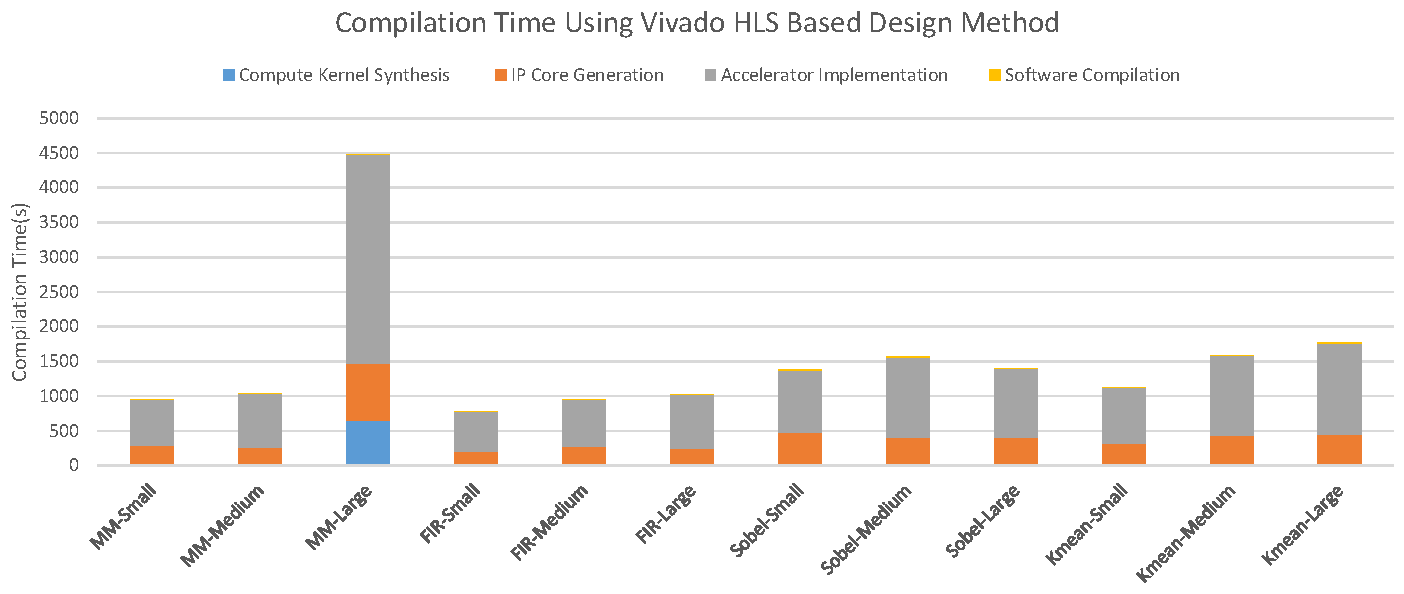
\includegraphics[width=0.95\linewidth]{HLS-Compilation-Time}}
\caption{Compilation Time Using Vivado HLS Based Design Method}
\label{fig:Vivado-HLS-Compilation-Time}
\end{figure}

\begin{figure}[H]
\center{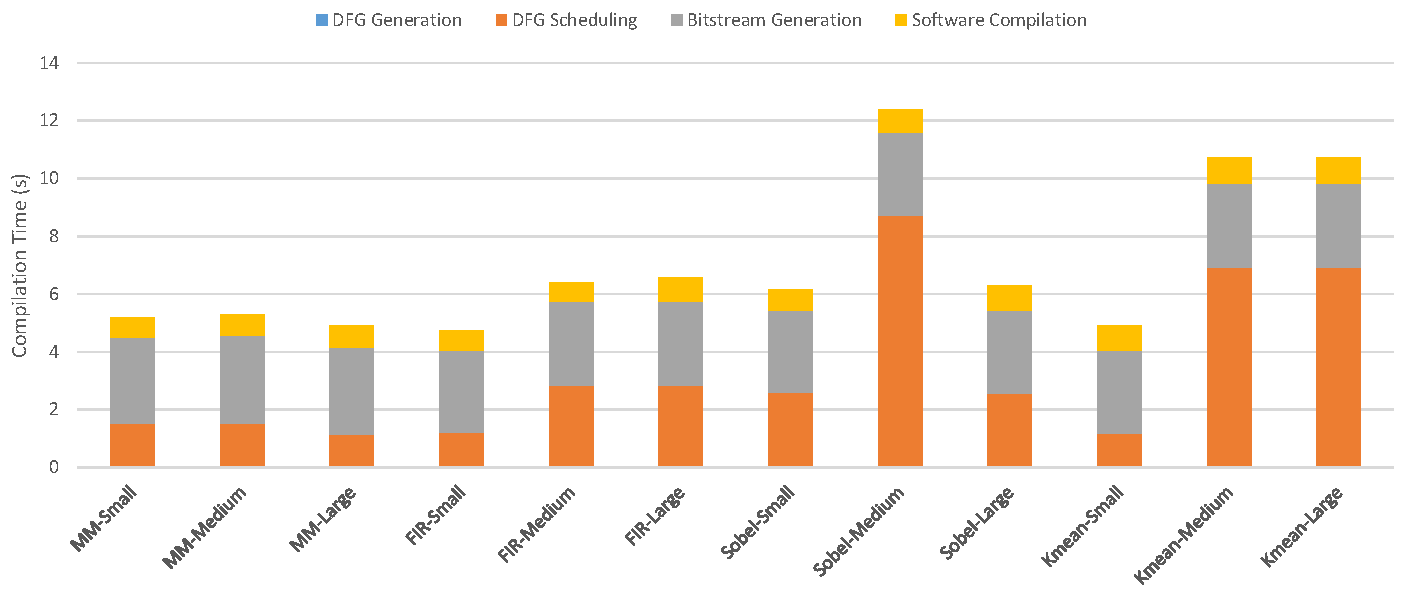
\includegraphics[width=0.95\linewidth]{QuickDough-Compilation-Time}}
\caption{Compilation Time Using SCGRA Overlay Based Design Method}
\label{fig:SCGRA-Overlay-Compilation-Time}
\end{figure}

\subsubsection{Hardware Implementation Efficiency}
In this section, hardware implementation efficiency including the hardware resource overhead, implementation frequency and implementation scalability using the two accelerator design methods are compared. 

\tabref{tab:hardware-overhead-comparison} exhibits the hardware overhead using both accelerator design methods. It is clear that Vivado HLS based accelrator typically consumes much less FF, LUT and RAM36 due to the delicate customization for each application configuration. However, the number of DSP48 required increases dramatically with the expansion of the application kernel which is mostly induced by loop unrolling. As a result, DSP48 can be the bottleneck that constrains the performance of the accelerator through loop unrolling. SCGRA based accelerator usually costs more FF, LUT and particularly RAM36 as expected, while the DSP consumtion scales linearly with the SCGRA size. Note that the hardware overhead using Vivado HLS based design method in this table refers to the configuration with fixed 2k-word input/output buffer. The overhead with maximum input/output buffer configuration doesn't change the conclusion here and is skipped to save the space. 

\begin{table}[h]
\centering
\caption{Hardware Overhead Using Both Vivado HLS and the SCGRA Based Accelerator Design Methods}
\label{tab:hardware-overhead-comparison}
\begin{tabular}{|l|l|l|l|l|l|}
\hline
\multicolumn{2}{|l|}{} & FF  & LUT & RAM36 & DSP48 \\ \hline
\multirow{3}{*}{MM}& Small & 5099 & 3730 & 4 & 102 \\ \cline{2-6} 
                   & Medium & 2778 & 3217 & 4 & 9 \\ \cline{2-6} 
                   & Large & 8282 & 10228 & 4 & 9 \\ \hline
\multirow{3}{*}{FIR}& Small & 5287 & 4494 & 4 & 99 \\ \cline{2-6} 
                   & Medium & 5283 & 4577 & 4 & 99 \\ \cline{2-6} 
                   & Large & 5283 & 4577 & 4 & 99 \\ \hline
\multirow{3}{*}{Sobel}& Small & 8503 & 6436 & 4 & 216 \\ \cline{2-6} 
                   & Medium & 6737 & 5526 & 4 & 144 \\ \cline{2-6} 
                   & Large & 6755 & 5546 & 4 & 144 \\ \hline
\multirow{3}{*}{KMean}& Small & 2852 & 3762 & 4 & 24 \\ \cline{2-6} 
                   & Medium & 5530 & 5427 & 4 & 24 \\ \cline{2-6} 
                   & Large & 5530 & 5427 & 4 & 24 \\ \hline
\multicolumn{2}{|l|}{SCGRA 2x2} & 9302 & 5745 & 32 & 4  \\ \hline
\multicolumn{2}{|l|}{SCGRA 5x5} & 34922 & 21436 & 137 & 25 \\ \hline
\multicolumn{2}{|l|}{FPGA Resource} & 106400 & 53200 & 140 & 220 \\ \hline
\end{tabular}
\end{table}

\figref{fig:impl-freq} shows detailed the implementation frequency of the benchmark using both FPGA accelerator design methods. Vivado HLS based accelerator works at most 100MHz on the Zedboard system due to the slow AXI controller. Even though the accelerator may work at individual clock domain, the synthesized IP core can also be slow especially when relatively larger loop unrolling is employed at high level language program synthesis step. While the SCGRA based is regular and it could works at higher clock domain. To make use of this advantage, the slow AXI controller block and the SCGRA are divided into two separate clock domains. Currently, SCGRA 2x2 works at 200MHz while SCGRA 5x5 works at 167MHz due to the high utilization of BRAM blocks. The controlling logic is slow and works at 100MHz.

\begin{figure}[H]
\center{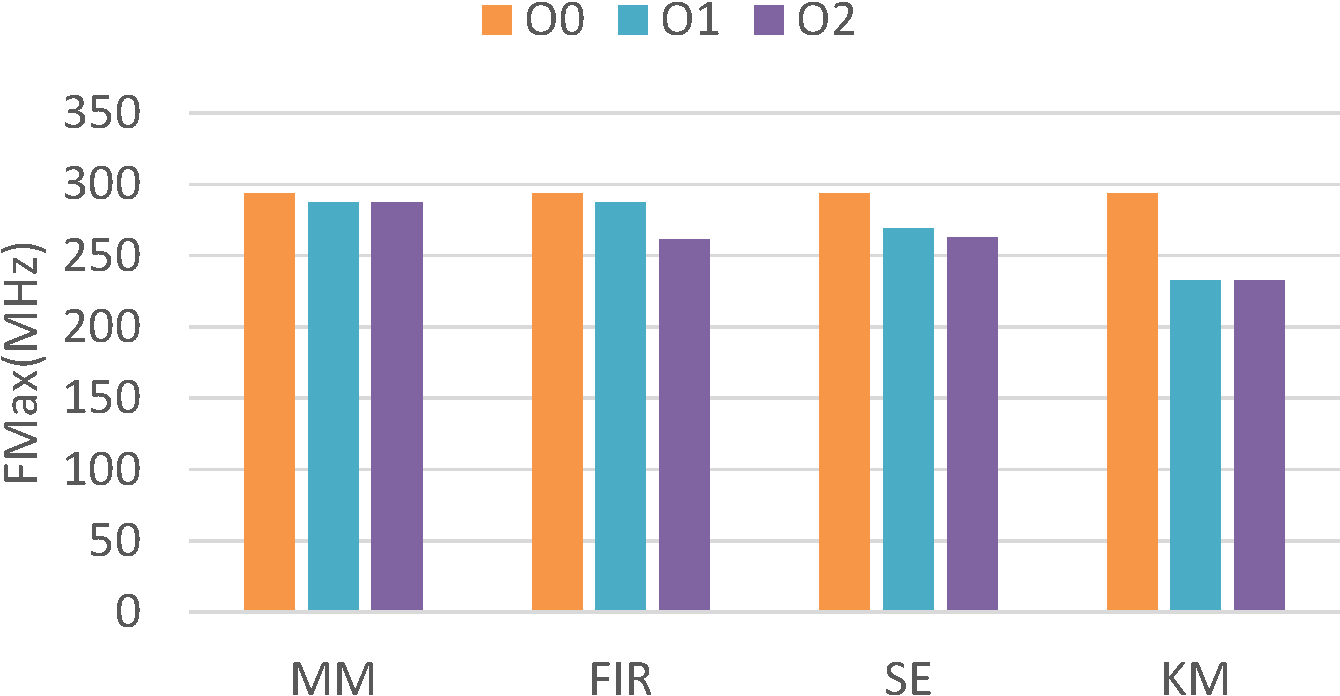
\includegraphics[width=0.95\linewidth]{impl-freq}}
\caption{Implementation Frequency of The Accelerators Using Vivado HLS and QuickDough}
\label{fig:impl-freq}
\end{figure}

When the application data set gets larger, both the accelerator design mathods may further scale the hardware infrastructure through loop unrolling and extending the SCGRA size etc. to accommodate the increased parallelism. Therefore, the scalability of the hardware implementation is also essential for the FPGA acceleration system. Figure xxx shows the implementation frequency of the accelerators kernel on xxx which could accommodate larger design than Zedboard. Since the implementation frequency of the Vivado HLS based accelerator depends on the specific application, we just use the simple matrix multiplication as an example. 

\subsubsection{Performance}
In this section, the execution time of the benchmark is taken as the performance metric. Since the execution time of different applications and data sets varies a lot, the performance speedup relative to Vivado HLS based implementation with 2k-Buffer is used instead. \figref{fig:real-perf} shows the performance comparison of four different sets of accelerator implementations including two SCGRA overlay based accelerators and two Vivado HLS based accelerators. According to this figure, Vivado HLS based design method wins the MM-Medium, MM-Large, Sobel-Medium and Sobel-Large, while QuickDough outperforms in FIR with all three data sets, Kmean-Medium and Kmean-Large. The two design methods achieve similar performance on the rest of the benchmark. 

\begin{figure}[H]
\center{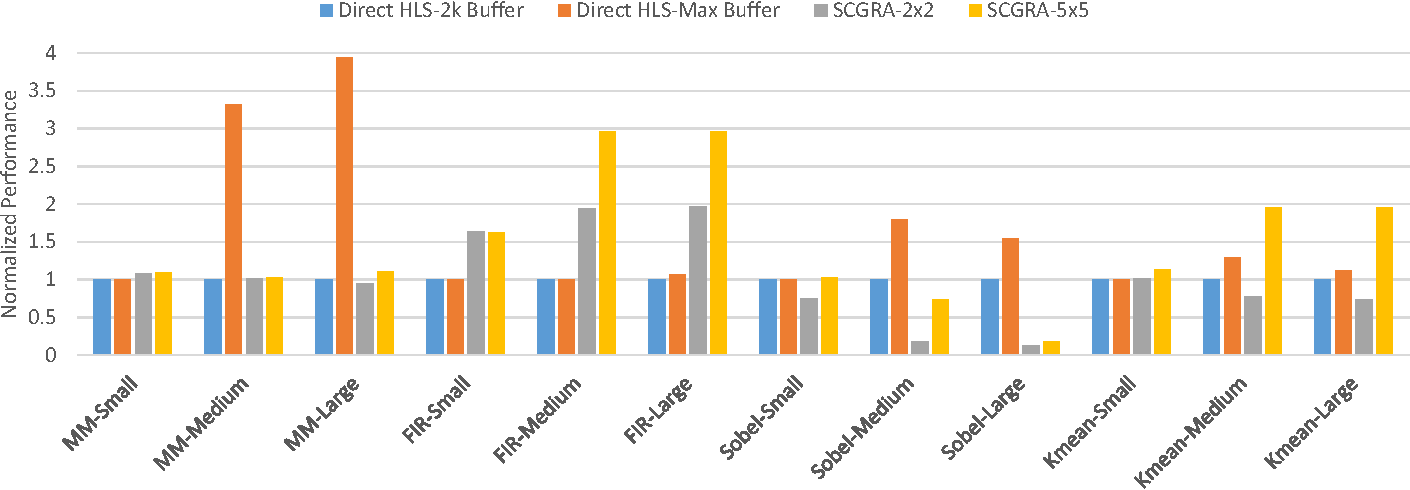
\includegraphics[width=0.95\linewidth]{real-perf}}
\caption{Benchmark Performance Using Both Vivado HLS Based Design Method and The SCGRA Overlay Based Design Method}
\label{fig:real-perf}
\end{figure}

To insight in the comparison of the two design methods, \figref{fig:execution-time} presents the execution time decomposition of the benchmark. As the benchmark runs on an ARM + FPGA system where FPGA handles the compute kernel leaving the rest on ARM processor, the execution of the benchmark can be roughly divided into four parts: system initialization such as DMA initialization, communication time between FPGA and ARM processor moving input/output data to/from the FPGA on-chip buffers, FPGA computation and the others such as input/output data reorganization for DMA transmission or corner case processing. The system initialization time is relatively small and is about the same for both design methods. The rest three parts determine the performance of different implementations. In addition, note that the execution time of different applications with diverse data sets varies in a large range. To fit all the data in a single figure, the execution time used in this figure is actually normalized to that of a basic software implementation on ARM. 

According to this figure, Vivado HLS based designs especially the designs with max-buffer configuration perform better performance mainly due to the smaller overhead in communication and others which are essentially the input/output data reorganization time. If we further look at the blocking details in \tabref{tab:loop-unrolling-setup-vivado}, it is clear that Vivado HLS based designs with max-buffer configuration could accommodate both larger data sets and corresponding computation, which could improve data reuse and deduce the amount of communication as well as data reorganization cost eventually. However, when there is little data reuse between the neighboring blocks, the design with larger data block couldn't reduce the amount of communication. Moreover, as the DMA is used to transmit the data between FPGA and Main Memory and it brings additional cost such as DMA setup, communication cost per data can be reduced when the data block per DMA transmission is larger. The benefit will be neglegible when the data set goes upto thousands and the additional DMA cost is amortized, while the exact numer depends on the platform. In all the applications of the benchmark with meidum and large data sets, Vivado HLS based designs especially the Max-Buffer configuration exihibit much smaller communication cost and data reorganization cost.

\begin{figure}[H]
\center{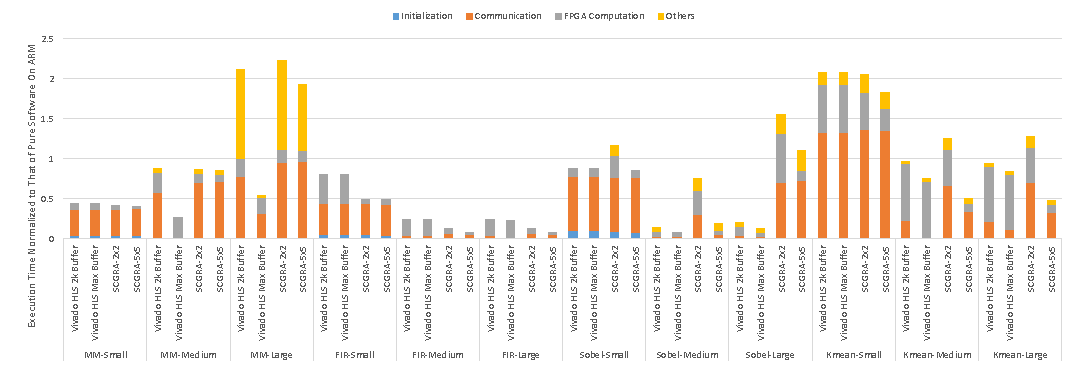
\includegraphics[width=0.95\linewidth]{execution-time}}
\caption{Implementation Frequency of The Accelerators Using Vivado HLS and QuickDough}
\label{fig:execution-time}
\end{figure}

Computation time is one of the most significant part of the overal execution time. It basically depends on both the simulation performance in cycles and implementation frequency of the hardware infrastructure. As explained in previous sections, QuickDOugh using SCGRA overlay has regular structure and could provide scalable and higher frequency hardware infrastructure. \figref{fig:kernel-sim-perf} shows the simulation performance which is the product of the block simulation performance and the number of blocks for each application. Apparently, QuickDough still fails to compete with the Vivado HLS based design in Sobel, but the performance gap of MM-Large is much smaller and particularly it shows better simulation performance on almost all the rest of the benchmark. The simulation performance comparison is quite relevant to the depth of the loop unrolling as shown in \tabref{tab:loop-unrolling-setup-vivado} and \tabref{tab:loop-unrolling-setup-scgra}. It indicates that the simulation performance depends heavily on the depth of the loop unrolling no matter HLS based customized circuit or SCGRA based overlay is used as the hardware infrastructure. While QuickDough using SCGRA overlay as the hardware infrastructure has advantages in terms of implementation freqeuncy, it enlarges its advatages in overall computation time as shown in \figref{fig:kernel-real-perf}. 

\begin{figure}[H]
\center{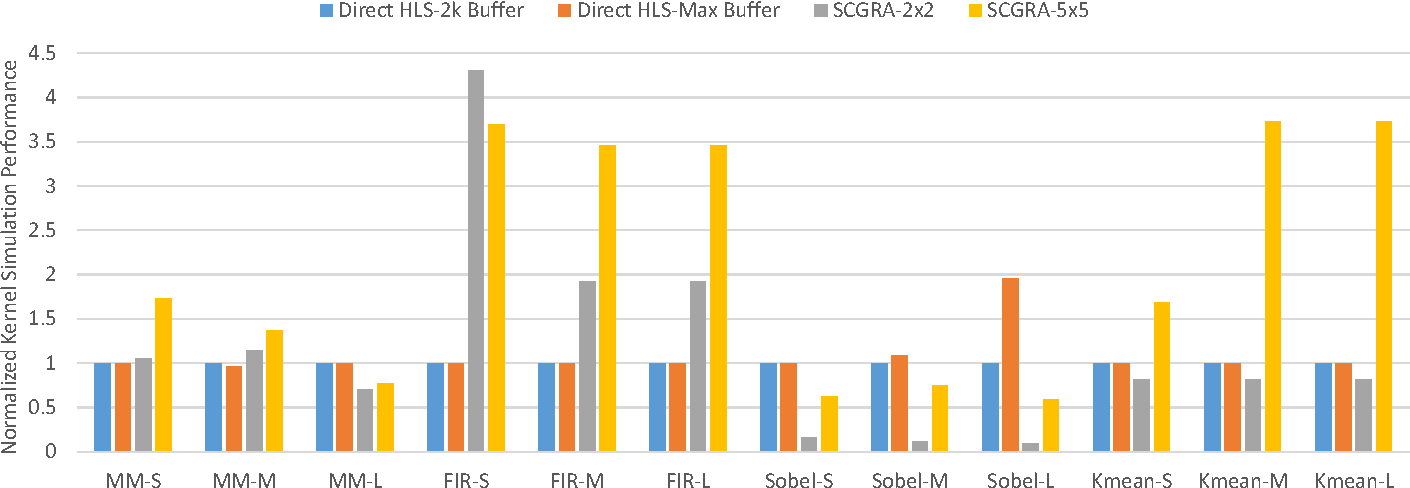
\includegraphics[width=0.95\linewidth]{kernel-sim-perf}}
\caption{Simulated Compute Kernel Performance Using Both Vivado HLS Based Design and QuickDough}
\label{fig:kernel-sim-perf}
\end{figure}

In summary, Vivado HLS based design could afford larger buffer and accommodate larger block size, which further helps to reduce the communication time and the cost of input/output organization. Therefore, when there are more data reuse among neighboring blocks, the Vivado HLS based design is able to achieve better performance. QuickDough using SCGRA overlay could provide both higher simulation performance with larger loop unrolling in many cases and higher implementation frequency due to its regular structure, so it will win when the target application has smaller data set and more compute intensive kernels.  

\begin{figure}[H]
\center{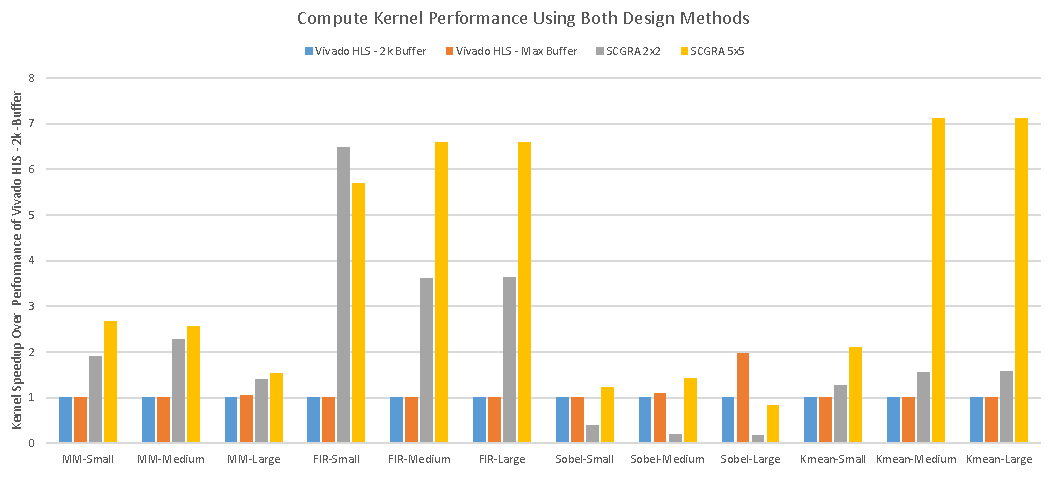
\includegraphics[width=0.95\linewidth]{kernel-real-perf}}
\caption{Compute Kernel Performance Using Both Vivado HLS Based Design and QuickDough}
\label{fig:kernel-real-perf}
\end{figure}
